\newpage
\section{Derivate}
\begin{definition}[Derivata]
    Dato un $A\subset \mathbb{R}$, una $f: A \to \mathbb{R}$, un $x_0 \in Acc(A) \cap A$. Se esiste il limite $\lim\limits_{x\to x_0}\frac{f(x) - f(x_0)}{x - x_0} = l$ allora $l$ si dice derivata di f in $x_0$. Se $l \in \mathbb{R}$ (è finito) allora $f$ si dice derivabile in $x_0$ la derivata si indica con $f'(x)$ oppure $Df(x_0)$, $\frac{df}{dx}(x)$, quindi:
    \begin{center}
        $f'(x_0) = \lim\limits_{x\to x_0}\frac{f(x) - f(x_0)}{x - x_0}$
    \end{center}
\end{definition}

\begin{figure}[h!]
    \vspace{-25pt}
    \centering
    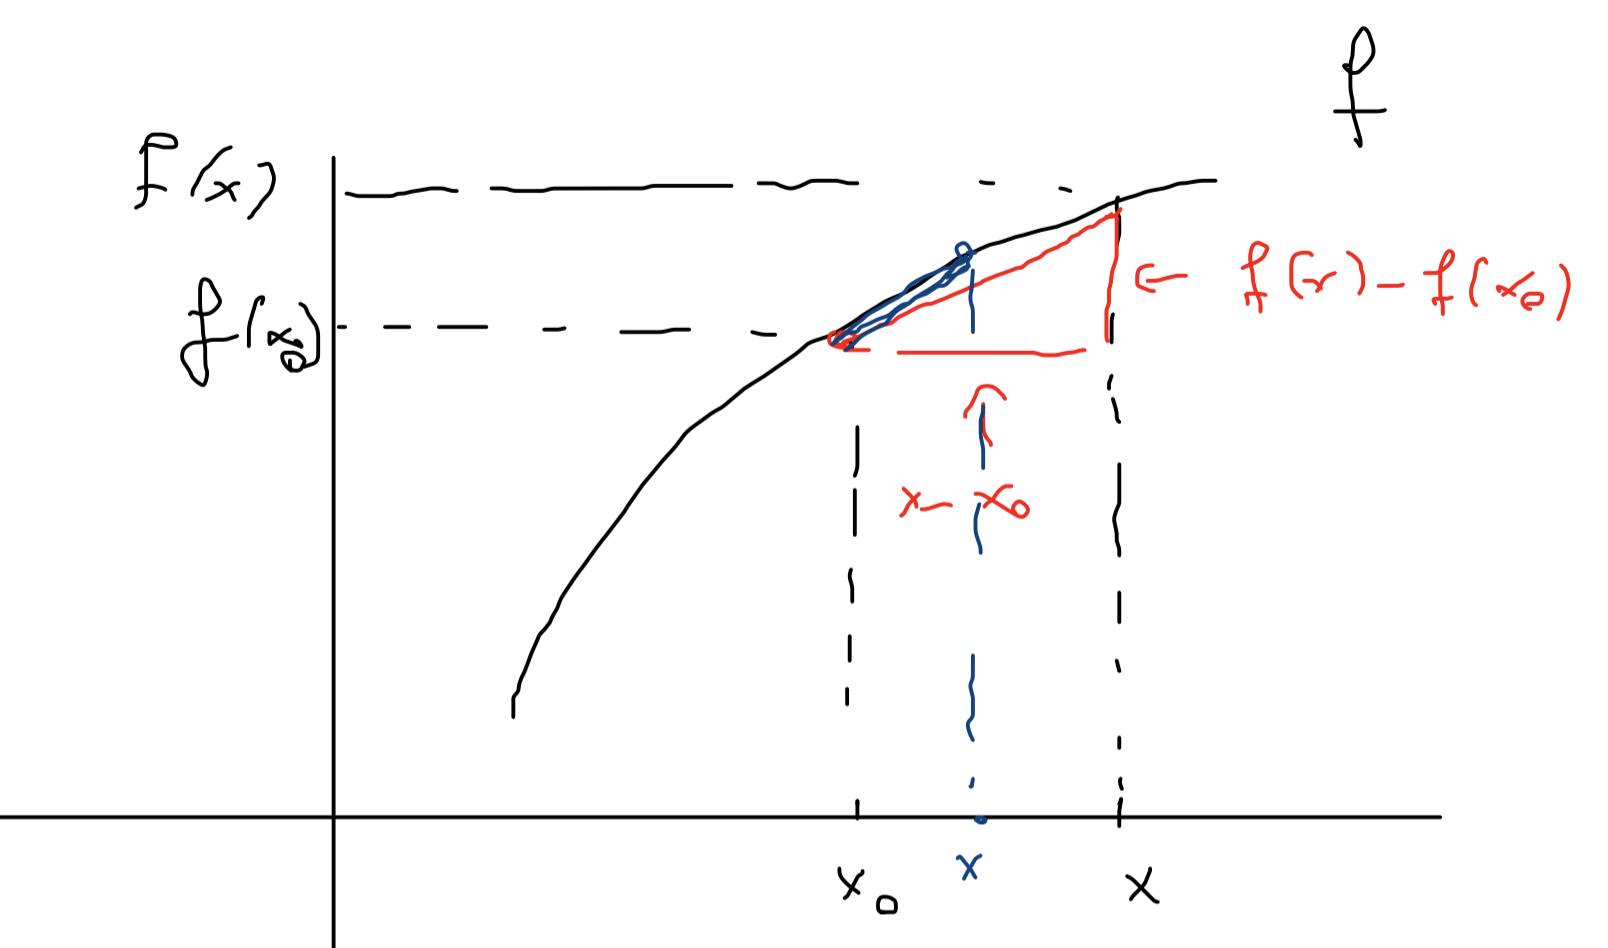
\includegraphics[width=10cm]{images/derivata-rapporto-incrementale.png}
    \vspace{-5pt}
    \caption{Derivata $f'(x_0) = \lim\limits_{x\to x_0}\frac{f(x) - f(x_0)}{x - x_0}$ con rapporto incrementale}
\end{figure}

\begin{observation}
Osserviamo che l'esistenza della derivata e la derivabilità sono due cose diverse perché la derivata potrebbe valere anche $\pm \infty$. In tal caso $f$ non è derivabile ma esiste la derivata
\end{observation}

\begin{example}
Prendiamo $f(x) = \sqrt{x}$ con $f: [0,+\infty) \to \mathbb{R}$. Calcoliamo al derivata in $x_0 = 0$.\\\\
$\lim\limits_{x\to 0}\frac{f(x) - f(0)}{x - 0} = \lim\limits_{x\to 0}\frac{\sqrt{x} - \sqrt{0}}{x - 0} = \lim\limits_{x\to 0}\frac{\sqrt{x}}{x} = \lim\limits_{x\to 0}\frac{1}{\sqrt{x}} = \frac{1}{0^+} = +\infty$.\\
$f'(0) = +\infty$ quindi $f$ non è derivabile in $x_0 = 0$
\end{example}

\subsection{Continuità funzioni derivabili}
\begin{theorem}[Continuità funzioni derivabili]
    Se prendiamo una $f$ che è derivabili in $x_0$ allora $f$ è continua in $x_0$
\end{theorem}
\begin{demostration}
Per dimostrare questo teorema proviamo a fare il $\lim\limits_{x \to x_0}f(x)$.\\
$\lim\limits_{x \to x_0}f(x) = \lim\limits_{x\to x_0}(f(x) - f(x_0) + f(x_0))$ (Andiamo a sommare e sottrarre una costante $f(x_0)$)\\\\
$= f(x_0) + \lim\limits_{x\to x_0}(f(x) - f(x_0))$ (Portiamo fuori una costante dal limite)\\\\
$= f(x_0) + \lim\limits_{x\to x_0}(\frac{f(x) - f(x_0)}{x - x_0}) \cdot (x - x_0))$ (Moltiplichiamo e dividiamo per $x - x_0$, otteniamo il rap. increm.)\\\\
$= f(x_0) + f'(x_0) \cdot \lim\limits_{x\to x_0} = f(x_0) + f'(x_0) \cdot 0 = f(x_0) + 0 = f(x_0)$ (Risolviamo il rap. increm.)\\\\
Allora $\lim\limits_{x\to x_0}f(x) = f(x_0)$ quindi $f$ è continua in $x_0$. $\blacksquare$
\end{demostration}

\begin{observation}
Possiamo però osservare che non è vero il contrario infatti se $f$ è continua non è detto che sia derivabile.
\end{observation}

\begin{example}
Facciamo un esempio per verificare questa osservazione. $f(x) |x|$ con $x_0 = 0$.\\
$\lim\limits_{x \to 0}\frac{f(x) - f(0)}{x - 0} = \frac{|x| - 0}{x - 0} = \frac{|x|}{x}$.
Ma abbiamo che $|x| = x$ con $x\geq 0$ e $|x| = -x$ se $x < 0$ quindi dobbiamo fare il limite destro e sinistro:
$\lim\limits_{x\to 0^+}\frac{|x|}{x} = \frac{x}{x} = 1$ e $\lim\limits_{x\to 0^-}\frac{|x|}{x} = \frac{-x}{x} = -1$.\\
Essendo diversi questi due limiti non esiste il limite e quindi non esiste la derivata di $|x|$ in $x_0 = 0$
\end{example} 

\subsection{Derivata destra e sinistra}
\begin{definition}[Derivata destra e sinistra]
    Se esiste $\lim\limits_{x\to x^+_0}\frac{f(x) - f(x_0)}{x - x_0}$ questa si chiama \textbf{derivata destra} di $f$ in $x_0$. Invece $\lim\limits_{x\to x^-_0}\frac{f(x) - f(x_0)}{x - x_0}$ si dice \textbf{derivata sinistra}. Si indicano con $f'_+(x_0)$ e $f'_-(x_0)$.
\end{definition}

\begin{observation}
Una funzione $f$ è derivabili in $x_0$ se e solo se $f'_+(x_0) = f'_-(x_0)$ e sono entrambi finite.
\end{observation}

\begin{example}
Facciamo un esempio di derivata destra e sinistra con $f(x) = |x|$ in $x_0 = 0$.\\
$f'_+(0) = 1$ mentre $f'_+(0) = -1$ quindi $f'_+(x_0) \neq f'_-(x_0)$ e quindi $f$ non è derivabile in $x_0 = 0$.
\end{example}

\subsection{Punto angoloso o di cuspide}
\begin{definition}[Punto angoloso]
    Se esiste $f'_+(x_0)$ e $f'_-(x_0)$ entrambi finite ma diverse tra loro allora $x_0$ si dice \textbf{punto angoloso}
\end{definition}
\begin{definition}[Punto di cuspide]
    Se $f'_+(x_0) = +\infty$ e $f'_-(x_0) = -\infty$ (o viceversa) il punto $x_0$ si dice \textbf{punto di cuspide}. 
\end{definition}

\begin{figure}[h!]
    \centering
    \begin{subfigure}{.4\textwidth}
        \centering
        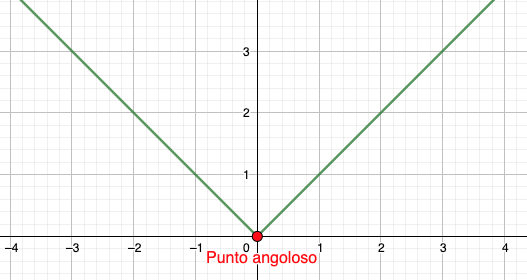
\includegraphics[width=6cm]{images/punto-angoloso.png}
        \caption{}
    \end{subfigure}
    \hspace{2cm}
    \begin{subfigure}{.4\textwidth}
        \centering
        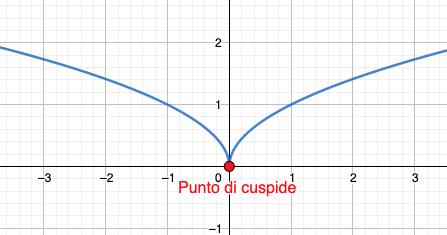
\includegraphics[width=6cm]{images/punto-cuspide.png}
        \caption{}
    \end{subfigure}
    \caption{In (a) un punto angoloso ed in (b) un punto di cuspide}
\end{figure}

\begin{example}
Prendiamo una $f(x) = \sqrt{|x|}$ con $f: \mathbb{R} \to \mathbb{R}$.
$f'_+(0) = +\infty$ mentre $f'_-(0) = -\infty$, quindi $f$ in $x_0 = 0$ ha un punto di cuspide.
\end{example}

\subsection{Retta tangente ad un punto}
\begin{observation}
$f$ è derivabile in $x_0$ se e solo se $f(x) = f(x_0) + f'(x_0) \cdot (x - x_0) + o(x - x_0)$.
$\lim\limits_{x\to x_0}\frac{f(x) - f(x_0)}{x - x_0} = f'(x_0)$ \\\\
$=\lim\limits_{x\to x_0}\frac{f(x) - f(x_0)}{x - x_0} - f'(x_0) = 0$ (Porto tutto dalla stessa parte)\\\\
$=\lim\limits_{x\to x_0}\frac{f(x) - f(x_0) - f'(x_0) \cdot (x - x_0)}{x - x_0} = 0$ (Porto tutto alla stesso denominatore)\\\\
$= f(x) - f(x_0) - f'(x_0) \cdot (x - x_0) = o (x - x_0)$ che è uguale $f(x) = f(x) + f(x_0) + f'(x_0) \cdot (x - x_0) + o (x - x_0)$.\\\\
La parte $f(x) + f(x_0) + f'(x_0) \cdot (x - x_0)$ ha un utilizzo particolare.
\end{observation}

\begin{definition}
    Se $f$ è derivabile in $x_0$ allora la retta $y = f(x_0) + f'(x_0) \cdot (x - x_0)$ si dice retta tangente al grafico di $f$ nel punto di coordinate $(x_0, f(x_0)$.
\end{definition}

\newpage
\subsection{Derivate di ordine superiori al primo}
$f: A \to \mathbb{R}$ supponiamo che $f$ sia derivabile in ogni punto $x \in A$. Allora $\exists f'(x) \forall x \in A$ e costituiscono la funzione derivata di $f$. $f': A \to \mathbb{R}$.\\\\
Se la funzione $f'$ è a sua volta derivabile posso calcolare la derivata che chiamo derivata seconda di $f$ ed indico con $f''$.\\
Posso in questo modo definire le derivate successive continuando a derivare le funzioni che otteniamo (se ovviamente sono derivabili).
\begin{example}
$f''(x) = (f')'$, $f'''(x) = (f'')'$, $f^(4)(x) = (f''')'$, ..., $f^{(n+1)}(x) = (f^{(n)})'$.\\
Per convenzione si indica con $f^{(0)}$ la funzione stessa $f^{(0)} = f$.
\end{example}

\begin{definition}
    Dato $n \in \mathbb{N}$ si dice che $f$ è di classe $C^n$ se $f$ è derivabile n-volte e $f^{(n)}$ è continua.
\end{definition}


\subsection{Operazioni sulle derivate}
\begin{theorem}
    Se $f,g$ sono funzioni derivabili in $x_0$ allora:
    \begin{enumerate}
        \item $f + g$ è derivabile in $x_0$ è vale che $(f + g)'(x_0) = f'(x_0) + g'(x_0)$.
        \item $f \cdot g$ è derivabile in $x_0$ e $(f \cdot g)'(x_0) = f'(x_0) \cdot g(x_0) + f(x_0) \cdot g'(x_0)$.
        \item Se $f(x_0) \neq 0$ allora $\frac{1}{f}$ è derivabile in $x_0$ e $(\frac{1}{f})'(x_0) = - \frac{f'(x_0)}{(f(x_0))^2}$ 
    \end{enumerate}
\end{theorem}

\begin{observation}
 Se $f,g$ sono derivabili in $x_0$ e $g(x_0) \neq 0$ allora andando a combinare il punto (2) e (3) del teorema sopra otteniamo che:
 \begin{center}\vspace{-5pt}
     $\frac{f}{g}$ è derivabile in $x_0$ e $(\frac{f}{g})'(x_0) = \frac{f'(x_0) \cdot g(x_0) - f(x_0) \cdot g'(x_0)}{(g(x_0))^2}$
 \end{center}
\end{observation}

\subsubsection{Derivata funzione inversa}
\begin{definition}[Derivabile della funzione inversa]
    Data una $f:(a,b) \to \mathbb{R}$ continua e strettamente monotona (quindi invertibile), se $f$ è derivabile in $x_0$ e $f'(x_0) \neq 0$ allora $f^{-1}$ è derivabile in $y_0 = f(x_0)$ ed è uguale a:
    \begin{center}
        $(f^{-1})'(y_0) = \frac{1}{f'(x_0)}$
    \end{center}
\end{definition}
\hspace{-15pt}Ricordiamo che $x_0 = f^{-1}(y_0)$ è possibile scriverlo come:
\begin{center}
    $(f^{-1})'(y_0) = \frac{1}{f'(f^{-1}(x_0))}$
\end{center}

\begin{example}
Facciamo un esempio con $f(x) = e^x$\\\\
$y = e^x \Longrightarrow x = \log(y) \Longrightarrow f^{-1}(y) = \log(y)$, quindi $f'(x) = e^x$\\\\
$(\log(y))' = (f^{-1}(y))' = \frac{1}{f'(f^{-1}(y))} = \frac{1}{e^{f^{-1}(y)}} = \frac{1}{e^{\log(y)}} = \frac{1}{y}$ con $y>0$ quindi la $D(\log(y)) = \frac{1}{y}$
\end{example}

\subsection{Derivate con funzione crescente e decrescenti}

\begin{proposition}
Prendiamo $A \subset \mathbb{R}$, una $f:A \to \mathbb{R}$ debolmente crescente in A. Se f è derivabile in un punto $x_0 \in A$ allora $f'(x_0) \geq 0$. Se $f$ è debolmente decrescente, e valgono le stesse condizione scritte prima, $f'(x_0) \leq 0$. 
\end{proposition}

\begin{demostration}
Prendiamo $f'(x_0) = \lim\limits_{x\to x_0} = \frac{f(x) - f(x_0)}{x - x_0}$. Ma se $f$ è debolmente crescente allora $\frac{f(x) - f(x_0)}{x - x_0} \geq 0$, ma visto che $f$ mantiene l'ordinamento, quindi numeratore e denominatore sono concordi in segno. A questo punto passando al limite si mantiene la disuguaglianza, quindi otteniamo che $f'(x_0) = \frac{f(x) - f(x_0)}{x - x_0} \geq 0$. $\blacksquare$
\end{demostration}

\begin{observation}
Se $f$ è strettamente crescente non posso dedurre che $f'(x_0) > 0$.  Ma solo che $f'(x_0) \geq 0$ questo perché quando passiamo al limite le disuguaglianze strette potenzialmente si indeboliscono, come visto nel teorema di confronto. 
\end{observation}

\begin{example}
Con $f(x) = x^3$ che è strettamente crescente in $\mathbb{R}$, abbiamo che $f'(x) = 3x^2$ e $f'(x) = 0$, quindi $f' \geq 0$ mentre $f > 0$ (la funzione "si indebolisce").
\end{example}

\subsection{Teorema di Fermat}
\begin{theorem}[Teorema di Fermat]
    $A \subset \mathbb{R}$, $f: A\to \mathbb{R}$. Se $x_0$ è un punto interno ad A che è di massimo o di minimo locale per $f$, e $f$ è derivabile in $x_0$, allora $f'(x_0) = 0$.
\end{theorem}

\begin{demostration}
Se $f$ è derivabile in $x_0$ allora $f'_+(x_0) = f'_-(x_0)$.\\
Supponiamo che $x_0$ sia punto di minimo locale per $f$, in un intorno di $x_0$ succederà che:\\\\
$f'_+(x_0) = \lim\limits_{x\to x_0^+}\frac{f(x) - f(x_0)}{x - x_0}$ dove $f(x) - f(x_0) \geq 0$ e $x - x_0 \geq 0$. Quindi $\frac{f(x) - f(x_0)}{x - x_0} \geq 0 \Longrightarrow f'_+(x_0) \geq 0$ \\\\
$f'_-(x_0) = \lim\limits_{x\to x_0^-}\frac{f(x) - f(x_0)}{x - x_0}$ dove $f(x) - f(x_0) \leq 0$ e $x - x_0 \leq 0 \Longrightarrow f'_-(x_0) \leq 0$. \\
Ma noi sappiamo che $f'_+(x_0) = f'_-(x_0) \Longrightarrow f'_+(x_0) = 0, f'_-(x_0) = 0 \Longrightarrow f'(x_0) = 0$
\end{demostration}

\begin{observation}
Osserviamo che se il punto non è interno al dominio allora il teorema non è necessariamente valido.
\end{observation}
\begin{example}
Prendiamo per esempio $f(x) = x^2$ ma definita come $f: [2,3] \to \mathbb{R}$ dove quindi il $min(f) = f(2) = 4$ ed il $max(f) = f(3) = 9$. Se calcoliamo la derivata abbiamo che $f'(x) = 2x$ e $f'(2) = 4$ ed ancora $f'(3) = 9$.
In questo caso 2 e 3 sono punti agli estremi del dominio e quindi non sono punti interni.
\end{example}

\begin{observation}
L'ipotesi di derivabilità è necessaria. Quindi possono esserci punti di minimo o di massimo locale dove la derivata non si annulla (perché non esiste).
\end{observation}
\begin{example}
Infatti se prendiamo la funzione $f(x) = |x|$ il punto $x = 0$ è punto di minimo assoluto (e quindi anche locale) ma la derivata $f'(0)$ non esiste.
\end{example}

\begin{observation}
Il teorema è condizione necessaria per un massimo o un minimo locale ma non sufficiente.
\end{observation}
\begin{example}
Prendiamo $f(x) = x^3$. $f'(x) = 3x^2$ ma $f'(x) = 0$ ma $x=0$ non è ne punti di massimo ne di minimo.
\end{example}

\subsection{Teorema di Rolle}
\begin{theorem}[Teorema di Rolle]
    Sia $f: [a,b] \to \mathbb{R}$ continua in [a,b] e derivabile in $(a,b)$.Se $f(a) = f(b)$ allora $\exists x \in (a,b)$ t.c. $f'(c) = 0$.
\end{theorem}

\begin{demostration}
Se $f$ è continua in $[a,b]$ per il teorema di Weirstrass assume massimo minimo. Siano $x_1$ e $x_2 \in [a,b]$ i punti di max e di min (2 dei possibili punti di massimo e minimo, essendo che possono essercene di più), cioè $f(x_1) = max(f)$ e $f(x_2) = min(f)$, distinguiamo 2 casi:
\begin{enumerate}
    \item $x_1 = a, x_2 = b$ o viceversa. Dato che $f(a) = f(b)$ allora sarebbe $max(f) = min(f)$ questo vuol dire che $f$ è costante in $[a,b] \Longrightarrow f'(x) = 0 \forall x \in (a,b)$
    \item Almeno uno dei due punti $x_1$ o $x_2$ non è negli estremi. Allora esiste un punto di massimo o di minimo interno ad (a,b), per il teorema di Fermat $f'(c) = 0$ (nel quale $x_1$ o $x_2$ uguale a $c$). $\blacksquare$
\end{enumerate}
\end{demostration}

\newpage
\subsection{Teorema di Lagrange}
\begin{theorem}[Teorema di Lagrange]
    Data una $f: [a,b] \to \mathbb{R}$, continua in $[a,b]$ e derivabile in $(a,b)$. Allora $\exists c \in (a,b)$ tale che:
    \begin{center}\vspace{-5pt}
        $f'(c) = \frac{f(b) - f(a)}{b - a}$
    \end{center}
\end{theorem}

\begin{demostration}
Definiamo una nuova funzione $r(x) = f(a) + \frac{f(b) - f(a)}{b - a}\cdot (x-a)$ che è una retta che passa per gli estremi del grafico, che sarebbero $(a,f(a))$ e $(b,f(b))$.\\
Definiamo anche $g(x) = f(x) - r(x)$, $g$ è continua in [a,b] e derivabile in (a,b).\\\\
$g(a) = f(a) - r(a) = f(a) - f(a) = 0$ \hspace{.5cm}$g(b) = f(b) - r(b) = f(b) - f(b) = 0$\\\\
Allora $g(a) = g(b)$ e quindi possono applicare Rolle alla funzione $g$. Quindi $\exists x \in (a,b)$ tale che $g'(c) = 0$. Calcoliamo ora $g'(x)$.\\\\
$g'(x) = f'(x) - r'(x) \:\:=\:\: f'(x) - \frac{f(b) - f(a)}{b - a}$.\\
Se $g'(c) = 0$ allora $f'(c) - \frac{f(b) - f(a)}{b - a} \Longrightarrow f'(c) = \frac{f(b) - f(a)}{b - a}$. $\blacksquare$
\end{demostration}

\subsubsection{Conseguenze del teorema di Lagrange}
\begin{theorem}
    Dato un $I \subset \mathbb{R}$ sia un intervallo $f: I \to \mathbb{R}$ continua in $I$ e derivabile nei punti interni di $I$ cioé in int(I). Allora valgono le seguenti affermazioni:
    \begin{enumerate}
        \item Se $f'(x) = 0 \forall x \in Int(I) \Longrightarrow f$ è contante in $I$.
        \item Se $f'(x) \geq 0 \forall x \in Int(I) \Longrightarrow f$ è debolmente crescente in $I$.
        \item Se $f'(x) \leq 0 \forall x \in Int(I) \Longrightarrow f$ è debolmente decrescente in $I$.
        \item Se $f'(x) > 0 \forall x \in Int(I) \Longrightarrow f$ è strettamente crescente in $I$.
        \item Se $f'(x) < 0 \forall x \in Int(I) \Longrightarrow f$ è strettamente decrescente in $I$.
    \end{enumerate}
\end{theorem}

\begin{demostration}
Dimostriamo il punto (4).\\
Prendiamo $x_1, x_2 \in I$ con $x_1 < x_2$. Devo dimostrare che $f(x_1) < f(x_2)$.\\\\
Visto $x_1$ o $x_2$ stanno in $I$ osservo che $(x_1,x_2) \subset Int(I)$. Allora applico il teorema di Lagrange all'intervallo $[x_1,x_2]$ (lo posso fare perché la funzione è continua in $[x_1,x_2]$ e derivabile in $(x_1,x_2)$).\\
Quindi $\exists c \in (x_1,x_2) $ tale che: $f'(x) = \frac{f(x_1) - f(x_1)}{x_2 - x_1}$.\\\\
Ma $f'(c) > 0 \Longrightarrow \frac{f(x_1) - f(x_1)}{x_2 - x_1} > 0$, quindi $f(x_2) - f(x_1) > 0$ (perché  $x_2 - x_1 > 0$ visto che $x_1 < x_2$) $\Longrightarrow f(x_2) > f(x_1)$. $\blacksquare$
\end{demostration}

\begin{observation}
Se $f$ non è definita su un intervallo il teorema potrebbe no essere vero.
\end{observation}

\begin{example}
$f(x) = \frac{1}{x}$ e $f: \mathbb{R} \setminus \{0\} \to \mathbb{R}$.\\
$f'(x) = -\frac{1}{x^2} < 0 \forall x \neq 0$, ma $f$ non è decrescente in $\mathbb{R} \setminus \{0\}$.\\
$f$ è strettamente decrescente in $(-\infty, 0)$ e in $(0, +\infty)$
\end{example}

\begin{example}
Prendiamo $f: (0, +\infty) \to \mathbb{R}$, $f(x) = \arctan(x) + \arctan\frac{1}{x}$ che è derivabile.\\
$f'(x) = \frac{1}{1 + x^2} + \frac{1}{1 + (\frac{1}{x})^2} \cdot (-\frac{1}{x^2}) \:\:\:=\:\:\: \frac{1}{1 + x^2} - \frac{1}{x^2 + 1} = 0 \Longrightarrow f$ è costante in $(0,+\infty)$.\\
Per calcolare la costante basta calcolare in un qualsiasi punto, per comodità prendiamo $x = 1$.\\
$f(1) = \arctan(1) + \arctan\frac{1}{1} = \frac{\pi}{4} + \frac{\pi}{4} = \frac{\pi}{2}$. Quindi $f(x) = \frac{\pi}{2}$ se $x > 0$ (visto che $x \in (0,+\infty)$).\\
Se $x < 0$ $f$ è costante perché $f'(x) = 0$ (va definita la funzione $f:(-\infty, 0) \to \mathbb{R}$).Per calcolare la costante valuto $f$ in $x = -1$.
$f(-1) = \arctan(-1) + \arctan\frac{1}{-1} = -\frac{\pi}{4} - \frac{\pi}{4} = -\frac{\pi}{2}$. \\Quindi $f(x) = -\frac{\pi}{2}$ se $x < 0$.\\
Questa seconda considerazione si poteva anche dedurre dal fatto che $f(x)$ è una funzione dispari.
\end{example}

\begin{proposition}
Dato un $I \subset \mathbb{R}$, una $f: A \to \mathbb{R}$, ed un $x_0 \in I$, $f$ derivabili in $I \setminus \{x_0\}$ e continua in $I$. Valgono (con $f'$ non necessariamente definita in $x_0$):
\begin{enumerate}
    \item Se $f'(x) \leq 0$ in un introno sinistro di $x_0$ e $f'(x) \geq 0$ in un intorno destro di $x_0$ allora $x_0$ è punto di minimo locale per $f$.
    \item Se $f'(x) \geq 0$ in un intorno sinistro di $x_0$ e $f'(x) \leq 0$ in un intorno destro  di $x_0$ allora $x_0$ è punto di massimo locale per $f$.
\end{enumerate}
\end{proposition}

\begin{example}
Data una $f(x) = x^3 - x$, $f: \mathbb{R} \to \mathbb{R}$.\\
$f'(x) = 3x^2 - 1$, studiamo il segno di $f'$:
$3x^2 - 1 \geq 0 \Longleftrightarrow 3x^2 \geq 1 \Longleftrightarrow x^2 \geq \frac{1}{3} \Longrightarrow |x| \geq \frac{1}{\sqrt{3}}$ cioè $x \in (-\infty, -\frac{1}{\sqrt{3}}] \cup [\frac{1}{\sqrt{3}}, +\infty)$
\end{example}

\begin{example}
Vediamo ora un caso in cui $f$ non sia derivabile in $x_0$.\\
$f(x) = |x|$ $f$ non è derivabile in $x_0 = 0$, $f'(x) = \begin{cases} 1 & se x \geq 0 \\ -1 & se x < 0\\\end{cases}$.\\\\
Avrò dunque che $x_0 = 0$ è punto di minimo anche se in quel punto la funzione non è derivabile.
\end{example}

\begin{example}
$f(x) = \sqrt{|x|}$, questa funzione ha una cuspide in $x = 0$, in questo punto quindi la funzione non è derivabile ma ugualmente il punto è un punto di minimo.
\end{example}

\begin{theorem}
    Dato $A \subset \mathbb{R}$, $f: A \to \mathbb{R}$, $x_0 \in Int(A)$, con $f$ derivabile 2 volte in $x_0$ e $f'(x_0) = 0$. Valgono allora le seguenti affermazioni:
    \begin{enumerate}
        \item Se $x_0$ è punto di minimo locale $\Longrightarrow f''(x_0) \geq 0$.
        \item Se $x_0$ è punto di massimo locale $\Longrightarrow f''(x_0) \leq 0$.
        \item Se $f''(x_0) > 0$ $\Longrightarrow$ $x_0$ è punto di minimo locale.
        \item Se $f''(x_0) < 0$ $\Longrightarrow$ $x_0$ è punto di massimo locale.
    \end{enumerate}
\end{theorem}
\begin{note}
In questo teorema le condizioni (1) e (2) sono \textbf{necessarie} mentre le (3) e (4) sono \textbf{sufficienti}.
\end{note}

\begin{example}
Dato $f(x) = x^2$ e $f'(x) = 2x$, $f''(x) = 2$, $f''$ è sempre $> 0$.\\
$f'(0) = 0$, $f''(x) > 0 \Longrightarrow x = 0$ è punti di minimo locale.
\end{example}

\begin{example}
Definiamo una $g(x) = - x^2$ e $g'(x) = -2x$, $g''(x) = -2$.\\
$g'(0) = 0$ e $g''(0) = -2 < 0 \Longrightarrow x_0 = 0$ è punto di massimo locale.
\end{example}

\begin{note}
Se $f''(x_0) = 0$ (la disuguaglianza quindi è debole) non posso affermare niente.
\end{note}

\begin{example}
Per verificare la nota prendiamo $h(x) = x^3$, $h'(x) = 3x^2$ e $h''(x) = 6x$.\\
$h'(0) = 0$, $h''(0) = 0$ ma $x_0 = 0$ non è ne di massimo ne di minimo locale.
\end{example}

\begin{example}
$f(x) = x^4$, $f'(x) = 4x^3$ e $f''(x) = 12x^3$.\\
$f(0) = 0$ e $f''(0) = 0$ e in questo caso $x_0 = 0$ è punto di minimo.\\
Mentre se prendo $g(x) = -x^4$ e $g'(0) = 0$ e $g''(0) = 0$ e quindi $x_0 = 0$ è punto di massimo.
\end{example}

\subsection{Teorema di Cauchy}
\begin{theorem}
    Siano $f,g: [a,b] \to \mathbb{R}$ continue in $[a,b]$ e derivabili in $(a,b)$. Allora $\exists c \in (a,b)$ t.c.
    \begin{center}
        $f'(c)(g(b) - g(a)) = g'(c)(f(b) - f(a))$
    \end{center}
    Se inoltre $g'(x) \neq 0 \forall x \in (a,b)$ allora la relazione precedente si può scrivere come:
    \begin{center}
        $\frac{f'(c)}{g'(c)} = \frac{f(b) - f(a)}{g(b) - g(a)}$
    \end{center}
\end{theorem}
Questa formula ci dice che c'è un punto in cui il rapporto delle derivate delle due funzioni in quel punto è uguale al rapporto degli incrementi totali delle funzioni sull'intervallo. Inoltre l'ipotesi $g'(x) \neq 0 \: \: \forall x \in (a,b)$ garantisce che non ci siano punti in cui la derivata prima si annulli.


\subsection{Teorema di de l'Hopital}
\begin{theorem}
    Siano $a,b \in \overline{\mathbb{R}}$, siano $f,g: (a,b) \to \mathbb{R}$ derivabili in $(a,b)$. Se valgono le seguenti condizioni:
    \begin{enumerate}
        \item $\lim\limits_{x\to a^+}f(x) = \lim\limits_{x\to a^+}g(x) = 0$ oppure $\lim\limits_{x\to a^+}f(x) = \pm\infty$ e $\lim\limits_{x\to a^+}g(x) = \pm\infty$.
        \item $g'(x) \neq 0$ in un introno destro di $a$.
        \item $\exists \lim\limits_{x\to a^+}\frac{f'(x)}{g'(x)} = l \in \overline{\mathbb{R}}$.
    \end{enumerate}
    allora $\exists \lim\limits_{x\to a^+}\frac{f(x)}{g(x)} = l$. (Stesso risulta con per $x \to b^-$)
\end{theorem}

\begin{note}
Questo teorema funziona anche nel caso di $x_0$ interno all'intervallo perché basta fare i due limiti destro e sinistro, e se coincidono otteniamo il limite complessivo.
\end{note}

\begin{example}
Facciamo un esempio per capire il funzionamento di questo teorema.\\\\
Calcoliamo $\lim\limits_{x\to 0}\frac{2\cos(x) - 2 + x^2}{x^4} = \frac{0}{0}$.\\
$f(x) = 2\cos(x) - 2 + x^2$ \: e \: $g(x) = x^4$ \hspace{.5cm} $f'(x) = -2\cos(x) + 2x$ \: e \: $g'(x) = 4x^3$\\
Provo a fare $\lim\limits_{x\to 0}\frac{f'(x)}{g'(x)} = \lim\limits_{x\to 0}\frac{-2\sin(x) + 2x}{4x^3} = \frac{0}{0}$, ancora indeterminato quini applico de l'Hopital. \\\\
$f(x) = -2\sin(x) + 2x$ e $g(x) = 4x^3$, quindi $f'(x) = -2\cos(x) + 2x$ e $g(x) 12x^2$\\\\
$\lim\limits_{x\to 0}\frac{-2\cos(x) + 2}{12x^2} = \frac{0}{0}$, ancora indeterminato quindi riapplico de l'Hopital.\\\\
$\lim\limits_{x\to 0}\frac{2\sin(x)}{24x} = \frac{1}{12}\lim\limits_{x\to 0}\frac{\sin(x)}{x} = \frac{1}{12} \cdot 1 = \frac{1}{12}$\\
\end{example}

\begin{example}
$\lim\limits_{x\to +\infty}\frac{e^x}{x^2} = \frac{+\infty}{+\infty}$, applico de l'Hopital derivando numeratore e denominatore.\\
$\lim\limits_{x\to +\infty}\frac{e^x}{2x} = \frac{+\infty}{+\infty}$, derivo di nuovo, $\lim\limits_{x\to +\infty}\frac{e^x}{2} = +\infty$.
\end{example}

\begin{observation}
Verificare sempre l'ipotesi (1) di de l'Hopital, cioè di essere una forma indeterminata.
\end{observation}

\begin{example}
$\lim\limits_{x\to 0}\frac{\cos(x)}{x^2} = \frac{1}{0^+} = +\infty$.\\
Se non mi accordo che l'ipotesi (1) non vale e applicando de l'Hopital (sbagliando) e derivo: $\lim\limits_{x\to 0}\frac{-\sin(x)}{2x} = -\frac{1}{2}$, sbagliano.
\end{example}

\begin{observation}
Potrebbe non esistere il $\lim\limits_{x\to x_0}\frac{f'(x)}{g'(x)}$ ma esistere il $\lim\limits_{x\to x_0}\frac{f(x)}{g(x)}$.
\end{observation}

\begin{example}
$f(x) = x^2\sin(\frac{1}{x})$ e $g(x) = x$.\\
$\lim\limits_{x\to 0}\frac{f'(x)}{g'(x)} = \lim\limits_{x\to 0}\frac{x^2 \sin(\frac{1}{x})}{x} = \frac{0}{0}$.
Se applico de l'Hopital e quindi derivo succede che: \\
$f'(x) = 2x\sin{\frac{1}{x}} + x^2\cos{\frac{1}{x}}\cdot(-\frac{1}{x^2}) = 2x\sin{\frac{1}{x}} - \cos{\frac{1}{x}}$ e $g'(x) = 1$\\\\
$\lim\limits_{x\to 0}\frac{f'(x)}{g'(x)} = \lim\limits_{x\to 0}\frac{2x\sin{\frac{1}{x}} - \cos{\frac{1}{x}}}{1}$ ma $2x\sin{\frac{1}{x}}$ tende a 0 mentre $- \cos{\frac{1}{x}}$ non esiste quindi il limite complessivamente non esiste.\\\\
Ma invece non uso de l'Hopital e faccio $\lim\limits_{x\to 0}\frac{f(x)}{g(x)} = \lim\limits_{x\to 0}\frac{x^2\cdot\sin{\frac{1}{x}}}{x} = 0$.\\
Quindi noto che in questo caso $\exists \lim\frac{f(x)}{g(x)}$ ma invece $\nexists \lim \frac{f'(x)}{g'(x)}$. Sarebbe quindi sbagliato dire che se $\nexists \lim \frac{f'(x)}{g'(x)} \Longrightarrow \nexists \lim \frac{f(x)}{g(x)}$.
\end{example}

\newpage
\begin{observation}
Se $\exists \lim\limits_{x\to x0}f(x) = l \in \mathbb{R}$ (limite finito), e $\nexists \lim\limits_{x\to x_0}g(x) \Longrightarrow \nexists \lim\limits_{x\to x_0}(f + g) = 0$.
\end{observation}
\begin{demostration}
Per assurdo se $\exists \lim\limits_{x\to x_0}(f + g)(x) = m$ allora $g(x) = (f + g)(x) - f(x)$ dove $(f + g)(x) \to m$ mentre $f(x) \to l$ quindi $g(x) = (f + g)(x) - f(x) \to m - l$ ma questo è assurdo perché $\nexists \lim\limits_{x\to x_0}g(x)$.
\end{demostration}

\begin{corollaries}
Se $f$ è continua in $x_0$ e derivabile in un intorno di $x_0$ (eccetto al più in $x_0$) e se esiste $\lim\limits_{x\to x_0}f'(x) = l \in \overline{\mathbb{R}} \Longrightarrow f'(x_0) = l$.
\end{corollaries}

\begin{example}
Prendiamo $f(x) = \begin{cases}x^2 + 1 & se \:\: x \geq 0\\ x^2 & se \:\: x < 0\\\end{cases}$. $f$ è derivabile in $x_0 = 0$?\\\\
$f'(x) = \begin{cases}2x & se \:\: x > 0\\ 2x & se \:\: x < 0\\\end{cases}$, (per ora non consideriamo 0).\\\\
$\lim\limits_{x\to 0^+}f'(x) = 0$ e $\lim\limits_{x\to 0^-}f'(x) = 0$, quindi $f$ non è derivabile in $x_0 = 0$ perché $f$ non è continua, e quindi non posso usare il corollario.
\end{example}

\begin{observation}
Se $\nexists \lim\limits_{x\to x_0}f'(x)$ non è detto che $f$ non sia derivabile in $x_0$.
\end{observation}

\begin{example}
$f(x) = \begin{cases}x^2\sin{\frac{1}{x}} & se \:\: x \neq 0\\ 0 & se \:\: x = 0\\\end{cases}$.\\
La funzione è continua in $x_0 = 0$ perché $\lim\limits_{x\to 0}x^2\sin{\frac{1}{x}} = 0 \cdot$ limitata $= 0 = f(0)$.\\
Vediamo se è derivabile:
\begin{enumerate}
    \item Calcolare il limite della derivata. Se $x \neq 0$ $f'(x) = 2x\sin{\frac{1}{x}} + x^2\cos{\frac{1}{x}} \cdot (-\frac{1}{x^2}) = 2x\sin{\frac{1}{x}} - \cos{\frac{1}{x}}$.\\
    $\lim\limits_{x\to 0}f'(x) = \lim\limits_{x\to 0}2x\sin{\frac{1}{x}} - \cos{\frac{1}{x}} = 0 - $ una cosa che non esiste $\Longrightarrow$ non esiste il limite di $f'(x)$. \\
    Da questo no posso concludere che $f$ non è derivabile in $x_0 = 0$.
    \item Limite del rapporto incrementale: $\lim\limits_{x\to 0}\frac{f(x) - f(0)}{x - 0} = \lim\limits_{x\to 0}\frac{x^2\sin{\frac{1}{x}} - 0}{x} = \lim\limits_{x\to 0}x\sin{\frac{1}{x}} = 0$. \\
    Quindi $f$ è derivabile e $f'(0) = 0$.
\end{enumerate}
\end{example}

\begin{example}
Esempio di de l'Hopital. \\
Calcoliamo $\lim\limits_{x\to 0^+}\frac{e^{-\frac{1}{x}}}{x^2} = \frac{e^{-\frac{1}{0^+}}}{0^+} = \frac{0}{0}$ e quindi posso usare de l'Hopital.\\
$\lim\limits_{x\to 0^+}\frac{e^{-\frac{1}{x}} \cdot (\frac{1}{x^2})}{2x} = \lim\limits_{x\to 0^+}\frac{e^{-\frac{1}{x}}}{2x^3}$, notiamo dunque che la situazione è peggiorata andando ad usare d l'Hopital rispetto a come si era partiti.\\
Possiamo osservare che $\frac{e^{-\frac{1}{x}}}{x^2} = \frac{\frac{1}{x^2}}{e^{\frac{1}{x}}} \to \frac{\infty}{\infty}$, riproviamo con de l'Hopital.\\
$\lim\limits_{x\to 0^+}\frac{\frac{1}{x^2}}{e^{\frac{1}{x}}}$ derivando viene che $\lim\limits_{x\to 0^+}\frac{\frac{-2}{x^3}}{e^{\frac{1}{x}} \cdot (-\frac{1}{x^2})} = \lim\limits_{x\to 0^+}\frac{2x^2}{e^{\frac{1}{x}} \cdot x^3} = \lim\limits_{x\to 0^+}\frac{\frac{2}{x}}{e^{\frac{1}{x}}}$, in questo caso la situazione è migliorata anche se è ancora indeterminato del tipo $\frac{\infty}{\infty}$, applico di nuovo de l'Hopital.\\
$\lim\limits_{x\to 0^+}\frac{-\frac{2}{x^2}}{e^{\frac{1}{x}} \cdot (-\frac{1}{x^2})} = \lim\limits_{x\to 0^+}\frac{2}{e^{\frac{1}{x}}} = \frac{2}{\infty} = 0$.
\end{example}

